%% ===================================================================
%% Appendix D. The Two-Sided Contraction Boundary
%% Full statement and proof of the bracket theorem (thm:cf2s_full), the
%% structural identities behind it, the first-order tightness figure, the
%% nonlinear-break conjecture (rem:obs_o1, kept as conjecture), and the
%% constants table. Labels app:bracket / thm:cf2s_full / eq:bracket_full /
%% rem:obs_o1 / tab:constants are referenced from the main text.
%% ===================================================================
\section{The Two-Sided Contraction Boundary}
\label{app:bracket}

\Cref{app:proof_phase} certified safety \emph{below} $\ecrit$. This section bounds the contraction
boundary from \emph{above} as well, proving the full version of \cref{thm:cf2s}: the budget at which
the operator first loses contraction sits between $\ecrit$ and a constant multiple of it. The lower
side holds for any $1$-Lipschitz $\phi$ and is the certificate the paper sells; the upper side is proved
for the all-active operator (A4), and the gap between them is a single computable constant. We work
under \cref{ass:tight-v2}, with $\Ahat$ symmetric and $\ecrit>0$.

\subsection{Two budgets and the gap between them}
\label{app:bracket-budgets}

Two budgets bound the boundary from opposite sides, the \emph{norm certificate} $\ecrit$ and the
\emph{all-active spectral break} $\espec$:
\begin{align}
\ecrit&=\frac{1-\kappa}{\norm{W}_2}=\frac{1}{\norm{W}_2}-\norm{\Ahat}_2,\\
\espec&=\frac{1}{\rho(W)}-\rho(\Ahat).
\end{align}
The certificate $\ecrit$ uses the operator norm $\norm{W}_2$, which is the worst case over all
directions, so it is conservative; the spectral budget $\espec$ uses the spectral radius $\rho(W)$,
which is the actual unstable direction, so it is exact for the all-active operator. The whole gap
between them is supplied by the nonnormality of $W$,
\begin{equation}
\espec-\ecrit=\Big(\tfrac{1}{\rho(W)}-\tfrac{1}{\norm{W}_2}\Big)+\big(\norm{\Ahat}_2-\rho(\Ahat)\big)\ \ge\ 0,
\label{eq:additive-gap}
\end{equation}
where the second bracket vanishes because $\Ahat$ is symmetric, leaving only the term driven by
$\gW:=\norm{W}_2/\rho(W)\ge1$.

The quantity $\gW$ is audited per model rather than controlled a priori: spectral normalization (A2)
caps $\norm{W}_2$ but not $\rho(W)$, so in principle $\rho(W)\to0$ at fixed $\norm{W}_2$ would send
$\gW\to\infty$. We therefore measure $\gW$ on each trained model ($\gW\in[1.19,2.47]$ on the suite,
with the a-posteriori certificate $\gW\le\kappa_2(V_W)$, the eigenvector conditioning of $W$) and report
the bracket constant as a function of that value. Every constant below is computable post-training from
$\rho(W),\norm{W}_2,\norm{\Ahat}_2$ and the edge set.

\subsection{Edge-feasible critical direction}
\label{app:bracket-align}

A break must be driven by a feasible perturbation, one that is symmetric and supported on existing
edges. Let $P_E$ be the orthogonal projection onto that subspace
$\mathcal S_E=\{M=M^\top:M_{ij}=0\text{ if }(i,j)\notin E\cup\{(i,i)\}\}$, let $u_1$ be a unit top
eigenvector of $\Ahat$, and set $g_E:=P_E(u_1u_1^\top)$, $\sigma_E:=\norm{g_E}_F$, and the unit feasible
direction $B:=g_E/\sigma_E$. The alignment of this feasible direction with the critical rank-one mode is
\begin{equation}
\beta:=\langle u_1,Bu_1\rangle=\frac{\langle u_1,P_E(u_1u_1^\top)u_1\rangle}{\sigma_E}
=\frac{\norm{g_E}_F^2}{\sigma_E}=\sigma_E,
\label{eq:beta-eq}
\end{equation}
using that $P_E$ is an orthogonal projection and $u_1u_1^\top$ is symmetric. So the alignment $\beta$
equals the edge-supported Frobenius mass $\sigma_E$ of the critical direction, which is strictly
positive whenever the Perron mode places mass on the edge set, true for every connected graph
($u_1>0$ entrywise, $E\ne\emptyset$). The hypothesis $\beta>0$ is therefore an observable, not an
assumption.

\subsection{The bracket theorem}
\label{app:bracket-thm}

\begin{theorem}[Constant-factor two-sided bracket for the all-active IGNN contraction boundary, full statement]
\label{thm:cf2s_full}
Let \cref{ass:tight-v2} hold with $\ecrit>0$ and $\Ahat$ symmetric, and let $\beta=\sigma_E\in(0,1]$ be
the edge-supported mass of the critical mode. Then:
\begin{enumerate}
\item[\textnormal{(i)}] \textbf{Lower side (any $1$-Lipschitz $\phi$).} For every feasible
$\delta\Ahat$ with $\norm{\delta\Ahat}_F\le\varepsilon<\eglob$, the perturbed operator is an
$\norm{\cdot}_2$-contraction with a unique equilibrium and $\rho(J_z')<1$, with no use of (A4); hence
$\ebreak\ge\eglob$. Under (A4), $\kappa=\norm{\Ahat}_2\norm{W}_2$ gives $\eglob=\ecrit$, so
$\ebreak\ge\ecrit$ and in particular $\ebreakall\ge\ecrit$.

\item[\textnormal{(ii)}] \textbf{Upper side (all-active, requires (A4)).} The feasible rank-one
$\delta\Ahat^\star=(\espec/\beta)\,B\in\mathcal S_E$, of size $\norm{\delta\Ahat^\star}_F=\espec/\beta$,
drives the all-active spectral radius to $1$, so $\ebreakall\le\espec/\beta$. In the
unconstrained-symmetric threat model ($P_E=I$, $\beta=1$) it is exact: $\ebreakall=\espec$ with
extremizer $\espec\,u_1u_1^\top$.

\item[\textnormal{(iii)}] \textbf{Constant-factor enclosure.} $\espec\le C\,\ecrit$ with the explicit,
dimension-free, a-posteriori-computable constant
\begin{equation*}
C:=\gW\,\frac{1+\kappa}{1-\kappa}
=\frac{\norm{W}_2}{\rho(W)}\cdot\frac{1+\norm{\Ahat}_2\norm{W}_2}{1-\norm{\Ahat}_2\norm{W}_2},
\end{equation*}
so the all-active boundary obeys
\begin{equation}
\boxed{\ \ecrit\ \le\ \ebreakall\ \le\ \tfrac{C}{\beta}\,\ecrit\ }.
\label{eq:bracket_full}
\end{equation}
The bracket is non-vacuous whenever $\beta>0$; on the suite $\beta\approx0.62$, giving
$C/\beta\lesssim16$. The $\beta$-free form $\ecrit\le\ebreakall\le C\,\ecrit$ holds exactly for the
unconstrained-symmetric model ($\beta=1$).

\item[\textnormal{(iv)}] \textbf{Equality conditions.}
(a) the endpoints coincide, $\ecrit=\espec$, iff $\gW=1$ ($W$ normal), independent of $\kappa,\beta$;
(b) all three coincide, $\ecrit=\ebreakall=\espec$, iff $\gW=1$ and $\beta=1$;
(c) the slack constant is one, $C/\beta=1$, iff additionally $\kappa\to0^+$.
\end{enumerate}
\end{theorem}

\begin{proof}
\emph{Setup.} Feasible perturbations lie in $\mathcal S_E$ with $\norm{\delta\Ahat}_F=\varepsilon$. We
use Weyl's inequality, $\rho(\Ahat')\le\rho(\Ahat)+\norm{\delta\Ahat}_2$ and
$\norm{\Ahat'}_2\le\norm{\Ahat}_2+\norm{\delta\Ahat}_2$, together with
$\norm{\delta\Ahat}_2\le\norm{\delta\Ahat}_F=\varepsilon$. Since $\Ahat$ and the extremal $\delta\Ahat$
are symmetric, $\rho(\Ahat')=\norm{\Ahat'}_2$ and Weyl holds with equality along an aligned rank-one
mode.

\emph{(i) Lower side.} By (A1) the activation mask is a $0/1$ projection, so exactly as in
\eqref{eq:Jzp-bound} $\norm{J_z'}_2\le(\norm{\Ahat}_2+\varepsilon)\norm{W}_2$ for \emph{every} mask, which
is below $1$ for $\varepsilon<\eglob$. A spectral-norm contraction has a unique fixed point and
$\rho(J_z')\le\norm{J_z'}_2<1$, so no feasible $\varepsilon<\eglob$ breaks contraction: $\ebreak\ge\eglob$,
using (A1)--(A3) only. Under the all-active operating point (A4) assumed for the upper side,
$\kappa=\norm{\Ahat}_2\norm{W}_2$, so $\eglob=\ecrit$ and $\ebreakall\ge\ecrit$. The additive gap
\eqref{eq:additive-gap} then gives $\ecrit\le\espec$.

\emph{(ii) Upper side, all-active.} Let $u_1$ be a unit top eigenvector of symmetric $\Ahat$. Along the
rank-one symmetric direction $t\,u_1u_1^\top$ ($\norm{u_1u_1^\top}_F=1$), $\rho(\Ahat+t\,u_1u_1^\top)=\rho(\Ahat)+t$
exactly, so under (A4), $\rho(J_z')=(\rho(\Ahat)+t)\rho(W)$ reaches $1$ at $t=\espec$, giving the
unconstrained break budget $\espec$ with extremizer $\espec\,u_1u_1^\top$. For edge feasibility, project
to $\mathcal S_E$ via $B=P_E(u_1u_1^\top)/\sigma_E$. The map
$t\mapsto\lambda_{\max}(\Ahat+tB)=\max_{\norm{v}=1}v^\top(\Ahat+tB)v$ is a pointwise maximum of affine
functions, hence convex, so it lies above its tangent at $t=0$,
$\rho(\Ahat+tB)\ge\rho(\Ahat)+\beta t$ for all $t\ge0$ (this lower direction is what convexity buys; a
concave version fails on every random instance). Choosing $\delta\Ahat^\star=(\espec/\beta)B$ drives
$\rho(\Ahat')\ge\rho(\Ahat)+\espec=1/\rho(W)$, so $\rho(J_z')\ge1$ and
$\ebreakall\le\norm{\delta\Ahat^\star}_F=\espec/\beta$, exact when $\beta=1$.

\emph{(iii) Closing the bracket.} Dropping $-\rho(\Ahat)\le0$ and using $\rho(\Ahat)=\norm{\Ahat}_2$,
$\espec\le1/\rho(W)=\gW/\norm{W}_2=\gW(\ecrit+\norm{\Ahat}_2)$. Since
$\norm{\Ahat}_2=\kappa/\norm{W}_2=\kappa(\ecrit+\norm{\Ahat}_2)$ gives
$\norm{\Ahat}_2=\tfrac{\kappa}{1-\kappa}\ecrit$, we obtain
$\espec\le\gW\tfrac{1}{1-\kappa}\ecrit\le\gW\tfrac{1+\kappa}{1-\kappa}\ecrit=C\,\ecrit$. With (i) and
(ii) the boxed bracket \eqref{eq:bracket_full} follows.

\emph{(iv) Equality conditions.} (a) The gap $\tfrac{1}{\rho(W)}-\tfrac{1}{\norm{W}_2}\ge0$ is zero iff
$\gW=1$, with $\kappa,\beta$ absent. (b) Adding edge-feasibility of the exact extremizer
$\espec\,u_1u_1^\top$ requires $\beta=1$, giving $\ecrit=\ebreakall=\espec$. (c) Forcing
$\tfrac{1+\kappa}{1-\kappa}=1$ in addition requires $\kappa\to0^+$.
\end{proof}

This recovers and sharpens \cref{thm:phase_transition}: the old result is the lower side (i), part (ii)
supplies the matching all-active upper side, and (iv) separates the three equality conditions. The
characterization is constant-factor (dimension-free), rate-sharp in the normal, edge-aligned corner
(iv)(b), with enclosure constant $C/\beta$ reaching $10$--$16\times$ on the suite (random-instance
$\espec/\ecrit\in[1.02,18.2]$, median $2.25$). Two identities, both numerically exact over thousands of
random certified-regime instances, underlie it: the all-active spectral law
$\rho(J_z')=\rho(\Ahat')\rho(W)$ (A4 only), and the additive gap \eqref{eq:additive-gap}, whose slack is
supplied entirely by $W$'s nonnormality when $\Ahat$ is symmetric.

\subsection{First-order tightness across the budget}
\label{app:bracket-tight}

The bracket rests on the first-order term being an accurate proxy for the true shift at the budgets we
use; \cref{fig:tightness_eps} confirms this directly. The ratio of the true equilibrium shift to its
first-order prediction stays within the operational budget and grows only as $\varepsilon$ leaves the
linear regime, which is exactly why the realistic-budget analysis below relies on the first-order
$\sigma_1(S_c)$ rather than on proximity to criticality.

\begin{figure}[t]
\centering
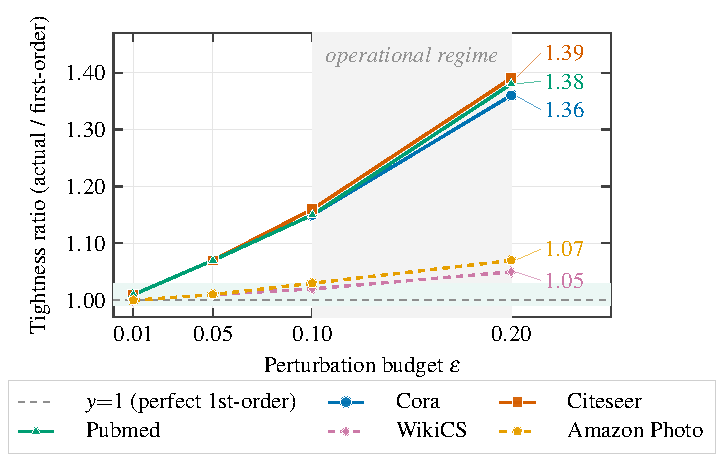
\includegraphics[width=\columnwidth]{figures/fig_tightness_eps.pdf}
\caption{First-order tightness of the equilibrium-shift prediction versus the perturbation budget
$\varepsilon$ (full graph, mean over 10 seeds). The ratio is the true shift divided by the first-order
prediction $\sigma_1(S)\varepsilon$; it is $1$ when the linearization is exact and rises as
$\varepsilon$ grows. Within the operational regime ($\varepsilon\le0.10$) every curve stays below
$1.16$; only at $\varepsilon=0.20$ do citation graphs (solid) reach $1.36$--$1.39$, while product graphs
(dashed) stay within $1.07$. This shift-prediction ratio is distinct from the ranking tightness quoted
elsewhere ($1.00$--$1.02$, \cref{app:explicit,app:ablations}), which is measured at the operational
subgraph scale; the figure traces the budget dependence that motivates capping $\varepsilon$ in that
regime.}
\label{fig:tightness_eps}
\end{figure}

\subsection{Nonlinear break budget: an empirical extension}
\label{app:bracket-o1}

\begin{remark}[Observation O1: nonlinear break budget and the active fraction; empirical, not part of \cref{thm:cf2s}]
\label{rem:obs_o1}
The deployed model is ReLU, not all-active, and its measured nonlinear break budget $\ereach$ exceeds
the all-active $\espec$. Over the 10 preferred seeds (50-node ego subgraph, $\norm{\Ahat}_F=1.77$): at
$\kappa_0=0.5$, $\ereach/\espec=1.41\pm0.12$ and $\ereach/\ecrit=2.17\pm0.18$; at $\kappa_0=0.9$,
$\ereach/\espec=1.51\pm0.18$ and $\ereach/\ecrit=8.72\pm1.03$. Empirically $\ereach\approx\espec/a$ with
$a$ the ReLU active fraction: $a\approx0.6$ gives $1/a\approx1.5$--$1.7$, matching the measured
$\ereach/\espec$, and composing with the bracket gives the observed envelope $\ereach/\ecrit\lesssim C/a$,
spanning roughly $[2,10]$.

\emph{This is a conjecture; two independent proof gaps remain open.} (1) \emph{Masked-operator spectral
scaling (unproved):} the relation $\ereach\approx\espec/a$ assumes the dominant eigenvalue of the masked
Jacobian $D_a(\Ahat'\otimes W)$ scales as $\approx a\,\rho(\Ahat')\rho(W)$, but no such lemma holds in
general because the active set correlates with the equilibrium and with $u_1$; this is a mean-field
heuristic calibrated to two operating points. (2) \emph{Linear-to-nonlinear bifurcation (empirical
only):} the step from ``a linearized eigenvalue reaches $1$'' to ``the true nonlinear fixed point
destabilizes'' is supported here only empirically across the 10 seeds (a clean simple-pole divergence,
critical exponent $\gamma\approx1.02$--$1.06$). We present $\ereach\approx\espec/a$ as an empirical
regularity organized by the same two knobs ($\gW$ and $a$), not a proven extension. The practical
consequence is benign: $\ereach$ runs $5$--$11\times$ the largest realistic budget ($\varepsilon\le0.2$),
so realistic-budget robustness is governed by the first-order $\sigma_1(S_c)$ of
\cref{fig:tightness_eps}, not by proximity to criticality.
\end{remark}

\begin{table}[t]\centering\footnotesize\setlength{\tabcolsep}{1pt}
\caption{Reconciliation of the robustness constants. The three ``$\times$'' ratios that recur in the
text are distinct quantities, not estimates of one number: the operating margin is how far the trained
model sits inside $\rho=1$, the empirical conservatism is how far $\ecrit$ under-states the true
nonlinear break, and the proven bracket is the worst-case enclosure constant.}
\label{tab:constants}
\begin{tabular}{@{}lll@{}}
\toprule
Quantity & Meaning & Source \\
\midrule
$\kappa=\norm{J_z}_2$ & trained contractivity ($<1$) & \cref{tab:cross_domain} \\
$\ecrit=\tfrac{1-\kappa}{\norm{W}_2}$ & norm certificate (safe radius) & \cref{thm:phase_transition} \\
$\espec$ & all-active spectral break budget & \cref{thm:cf2s} \\
$\mathbf{2}$--$\mathbf{4\times}$ & operating $\rho$-margin to $\rho=1$ & \cref{app:phase_scal} \\
$\mathbf{2}$--$\mathbf{9\times}$ & empirical $\ereach/\ecrit$ (10 seeds) & \cref{rem:obs_o1} \\
$\mathbf{10}$--$\mathbf{16\times}$ & proven bracket constant $C/\beta$ & \cref{thm:cf2s} \\
$\gamma\approx1.02$ & resolvent critical exponent & \cref{rem:obs_o1} \\
$\gW\in[1.19,2.47]$ & nonnormality $\norm{W}_2/\rho(W)$ & \cref{thm:cf2s} \\
\bottomrule
\end{tabular}
\end{table}
